\documentclass[10 pt,usenames,dvipsnames, oneside]{article}
\usepackage{../../../modelo-ensino-medio}



\begin{document}

\begin{center}
  \begin{minipage}[l]{3cm}

\includegraphics[width=2cm]{logo}    
\end{minipage}\hfill
\begin{minipage}[r]{.8\textwidth}
 {\Large \scshape Atividade: Duas exponenciais}  
\end{minipage}
\end{center}
\vspace{.2cm}

\ifdefined\prof
%Habilidades da BNCC
\begin{objetivos}
\item \textbf{EM13MAT403} Comparar e analisar as representações, em plano cartesiano, das funções exponencial e logarítmica para identificar as características fundamentais (domínio, imagem, crescimento) de cada uma, com ou sem apoio de tecnologias digitais, estabelecendo relações entre elas.
\end{objetivos}

%Caixa do Para o Professor
\begin{goals}
%Objetivos específicos
\begin{enumerate}
	\item Reconhecer o padrão exponencial em tabelas e gráficos;
	\item Identificar o fator de decrescimento e reconhecer o papel que ele desempenha.
\end{enumerate}

\tcblower

%Orientações e sugestões
\begin{itemize}
	\item Havendo disponibilidade utilize uma calculadora gráfica para explorar junto com a turma as características observadas nos gráficos associados a cada uma das expressões.
\end{itemize}
\end{goals}

\bigskip
\begin{center}
{\large \scshape Atividade}
\end{center}
\fi

Construa tabelas e gráficos para comparar os valores da variável $y$ nas duas expressões exponenciais para valores inteiros da variável $x$ de $1$ até $10$.

\[
y=2 \cdot 3^{x}  \text{ e } y=64 \cdot (1{,}5)^{x}.
\]

\begin{enumerate}

\item{}
Em qual das duas $y$ cresce a uma taxa maior? Como você sabe?

\item{}
Para que valor de $x$, os valores de $y$ coincidem? Como isso se reflete na representação gráfica?


\end{enumerate}

\ifdefined\prof
\begin{solucao}

\begin{table}[H]
	\centering

	\begin{tabu} to \textwidth{|>{$}c<{$}|>{$}c<{$}|}
	\hline
	\tnumber
	\bm{x} & \bm{2\cdot3^x} \\
	\hline
	1 & 6 \\
	\hline
	2 & 18 \\
	\hline
	3 & 54 \\
	\hline
	4 & 162 \\
	\hline
	5 & 486 \\
	\hline
	6 & 1458 \\
	\hline
	7 & 4374 \\
	\hline
	8 & 13122 \\
	\hline
	9 & 39366 \\
	\hline
	10 & 118098 \\
	\hline
	\end{tabu}\hspace{1em}
	\begin{tabu} to \textwidth{|>{$}c<{$}|>{$}c<{$}|}
	\hline
	\tnumber
	\bm{x} & \bm{64\cdot(1{,}5)^x} \\
	1 & 96 \\
	\hline
	2 & 144 \\
	\hline
	3 & 216 \\
	\hline
	4 & 324  \\
	\hline
	5 & 486 \\
	\hline
	6 & 729 \\
	\hline
	7 & 1093{,}5 \\
	\hline
	8 & 1640{,}25 \\
	\hline
	9 & 2460{,}375 \\
	\hline
	10 & 3690{,}5625 \\
	\hline
	\end{tabu}
	\end{table}
	\begin{figure}[H]
	\centering
	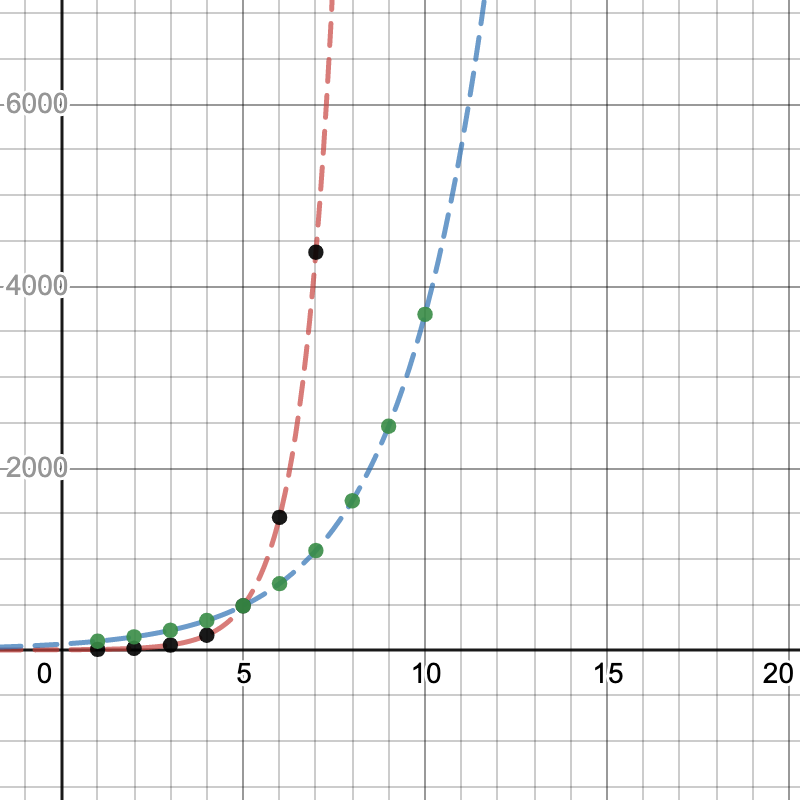
\includegraphics[width=200bp]{Duas_exponenciais.png}
	\end{figure}

	\begin{enumerate}
	\item{}
	$y$ cresce com maior taxa na segunda expressão. As tabelas acima mostram  que os valores correspondentes de $x$ retornam sempre valores de $y$ maiores ou iguais para a segunda expressão.

	\item{}
	$x=5$. Neste ponto os gráficos se interceptam.
	\end{enumerate}

\end{solucao}
\fi

\end{document}